\chapter{Conclusions}

\begin{figure}
\begin{centering}
\subfigure{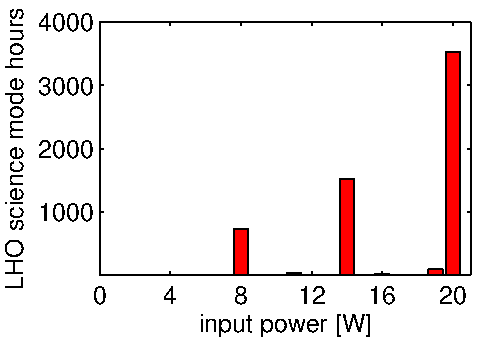
\includegraphics{figures/thesisS6pwrs_LHO.pdf}}\subfigure{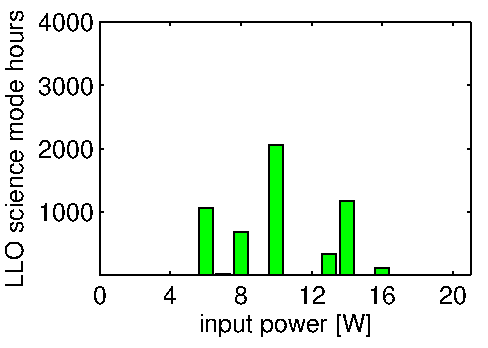
\includegraphics{figures/thesisS6pwrs_LLO.pdf}}
\caption[Histogram of input powers used during S6]{Histogram of input
  powers used during S6 at each site.}
\label{fig:S6pwrs}
\end{centering}
\end{figure}

We described the design of the Enhanced LIGO Input Optics and Angular
Sensing and Control subsystems and presented measurements
characterizing the systems and their performances when operating with
record laser powers. Upgrades to the two systems were necessary for
allowing higher laser powers, for improving the efficiency of sending
light into the interferometer, and for keeping light in the
interferometer once it is there. Higher power in the interferometer
improves the shot-noise-limited noise floor, and we succeeded at
operating the interferometers with more than twice the highest of
powers achievable during Initial LIGO, as shown by the histograms in
Fig.~\ref{fig:S6pwrs}. The Enhanced LIGO shot-noise-limited
sensitivity did indeed reach record levels, improving the chances
of gravitational-wave detection.

In addition, we directly measured the stable and unstable
opto-mechanical modes of the Fabry-P\'{e}rot arm cavities. We witness
the expected effect of radiation pressure torque, demonstrating a
clear understanding of the physics that will affect future generations
of laser interferometers for gravitational-wave
detection. Furthermore, we successfully controlled the stable and
unstable opto-mechanical modes without contaminating the
gravitational-wave readout in the frequency range of interest.


\begin{figure}
\begin{centering}
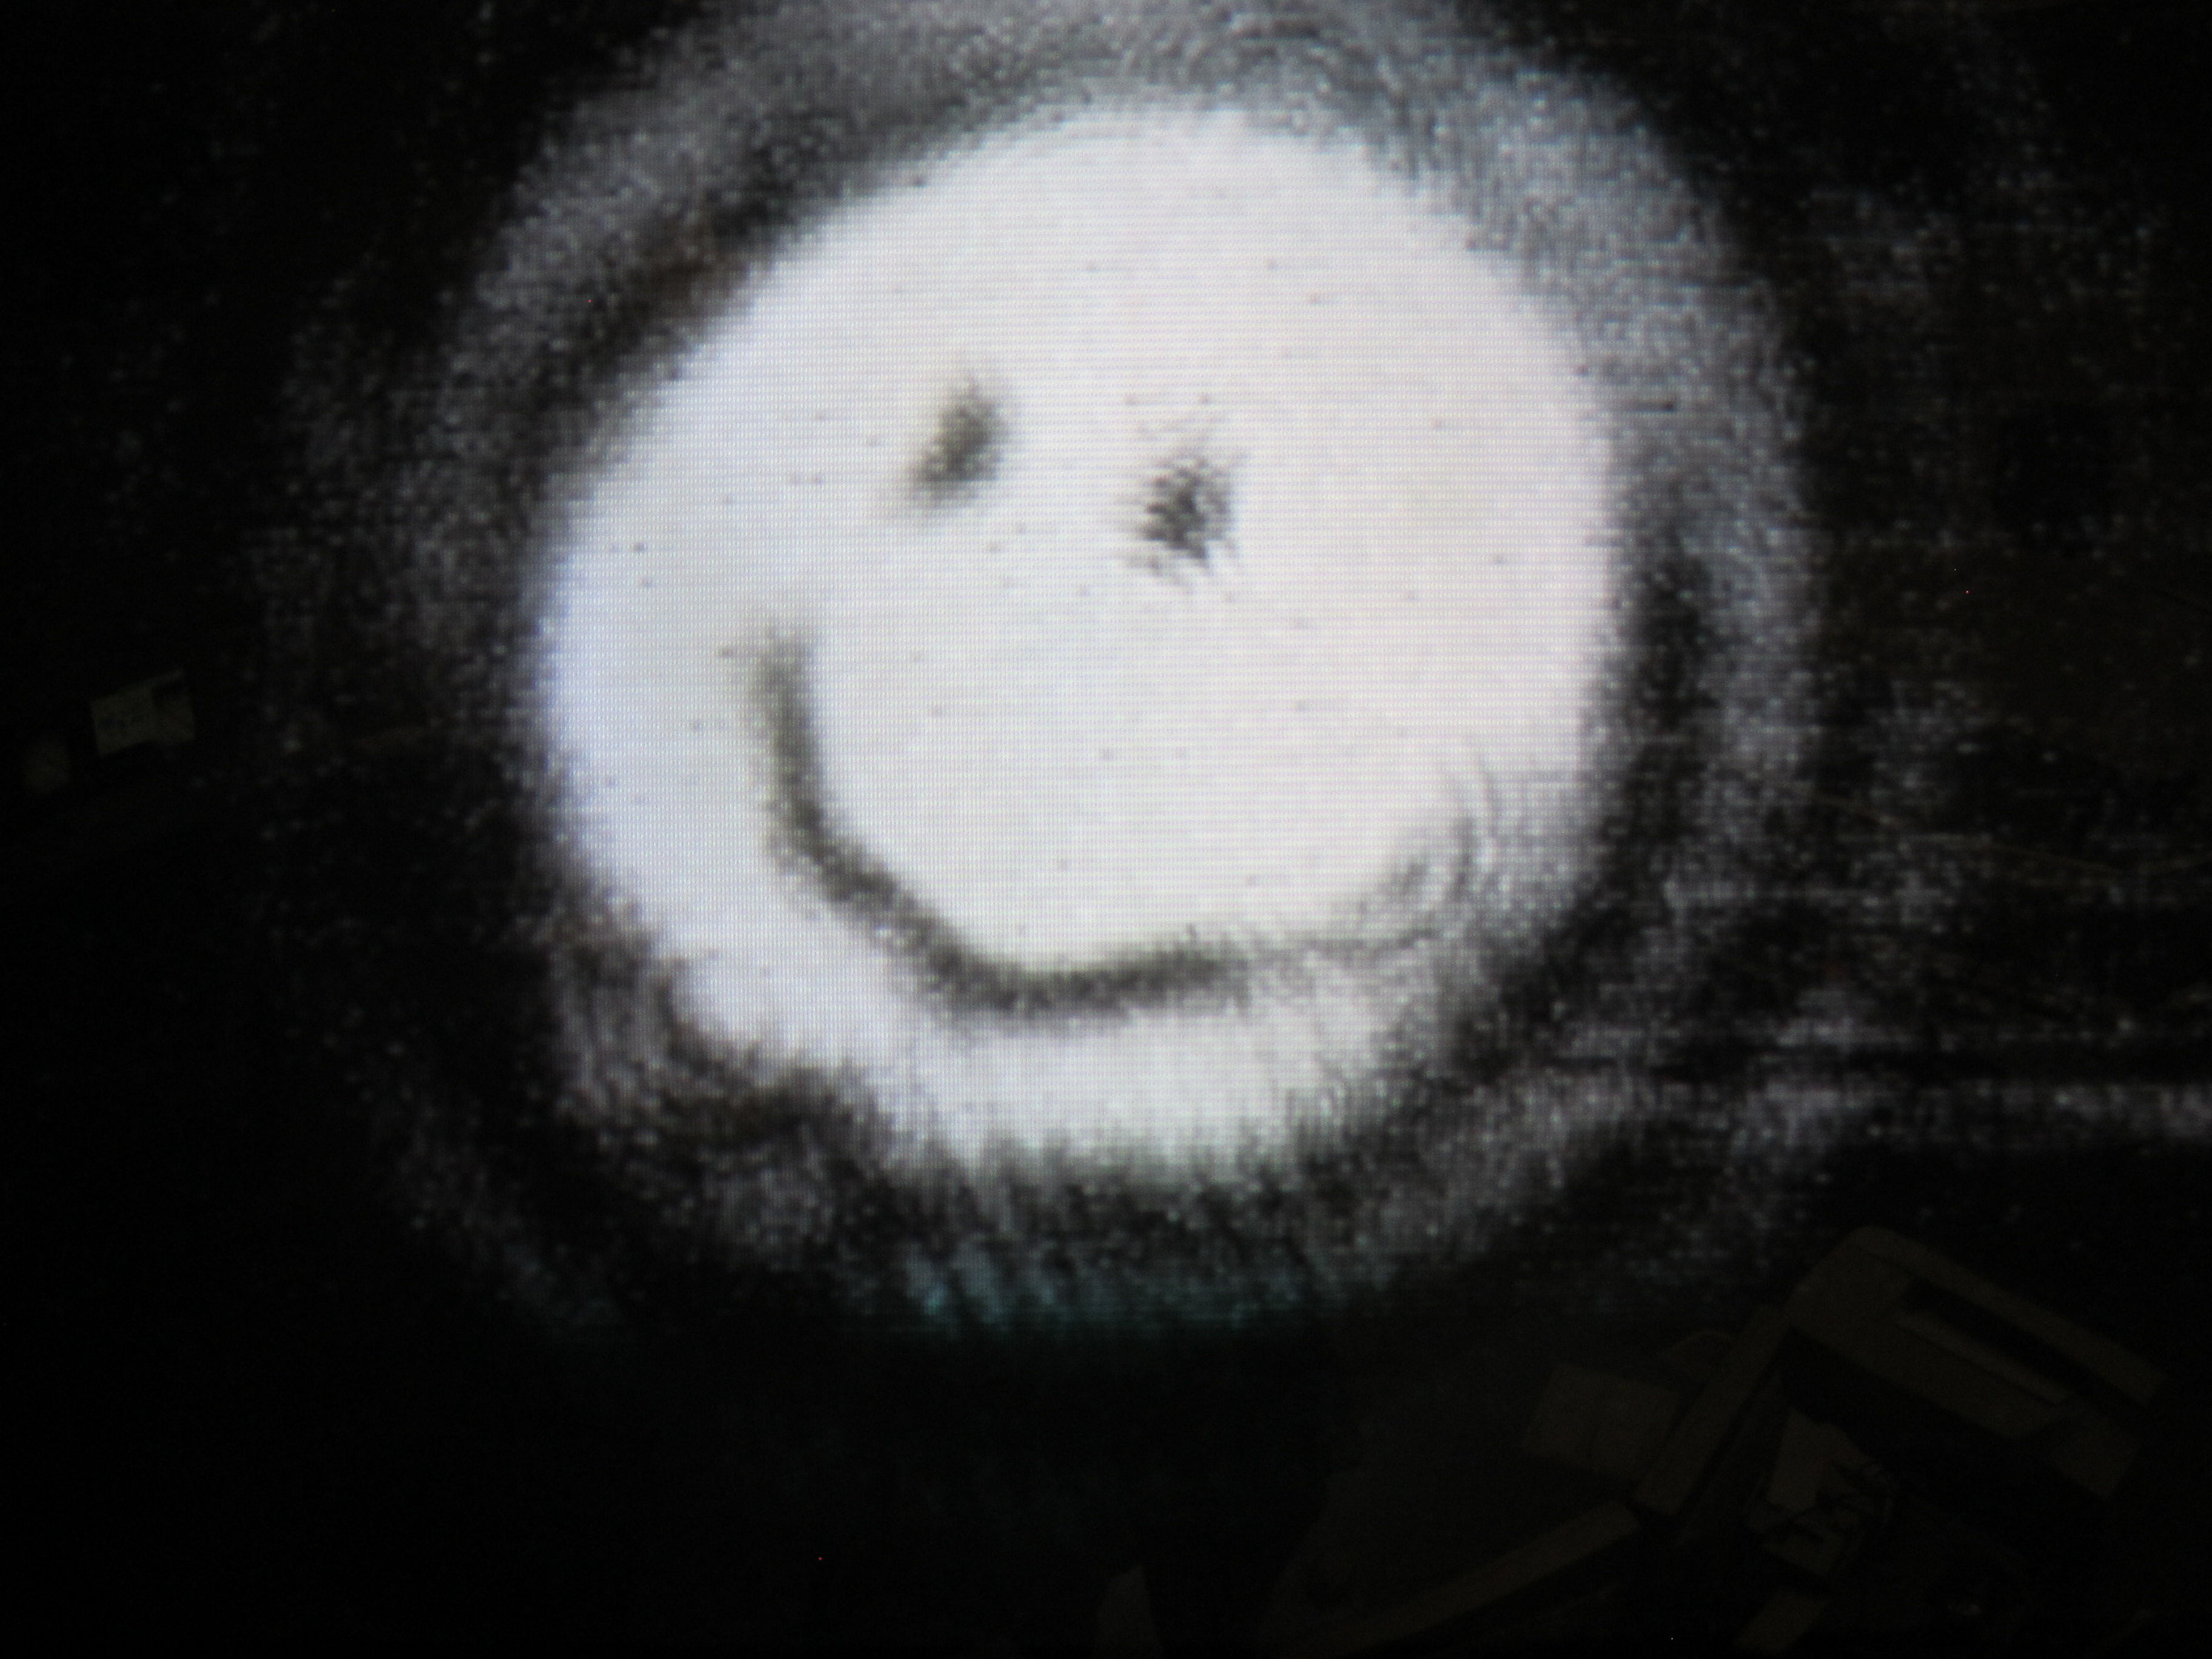
\includegraphics[width=0.8\textwidth]{figures/PMCRefl_smiley.JPG}
%\caption{Reflected beam from the Advanced LIGO pre-mode cleaner.}
\label{fig:smiley}
\end{centering}
\end{figure}


%\the\columnwidth